\documentclass[]{beamer}
\usetheme{KUL}
\usepackage{multirow}
\usepackage{multicol}
\usepackage{tikz}
\usepackage[normalem]{ulem}
%\usepackage[british]{babel}
% \usepackage{siunitx}
\newcommand\itemS{\item[\textbf{\S}]}
\definecolor{darkgreen}{rgb}{0,0.598,0.199}
\usepackage{times} % set font on times new roman
\usepackage{eurosym} % package for Euro sign
\usepackage{lineno}   % package for line numbering
\usepackage{hyperref} % this is for url links
\usepackage{subcaption}  % this package enables one to put several figures next to each other
\usepackage{textcomp}
\usepackage{setspace}
\usepackage{gensymb}
\usepackage{ dsfont }
\usepackage{changepage}
\usepackage{hyperref}
% \usepackage{biblatex}
% \addbibresource{bronnen.bib}

\usepackage{cancel}


\newcommand{\temp}[1]{\cancel{#1}} % {\kleur{#1}}

\usepackage{yarpackage}

\newenvironment{nonumberframe}{
    \setbeamertemplate{footline}{}
    \begin{frame}[c,noframenumbering]
    }{
    \end{frame}
    \setbeamertemplate{footline}{\hfill \color{black!85}\insertframenumber \hspace*{6mm}\vspace*{3pt}}
}

%% 

\AtBeginSection[]
{ 
  \begin{nonumberframe}
    \frametitle{Table of Contents}
    \tableofcontents[currentsection]
  \end{nonumberframe}
}

%----------------------------------
% Fill in the essential Information
%----------------------------------

\title[Meeting 1]{Master Thesis Meeting 1}
\author[Yarne]{Yarne Thijs}
\date{12/07/2024}
\institute[KU Leuven]{Faculty of Science\\ Master Of Mathematics}

%----------------------------------
% ACTUAL PRESENTATION STARTS HERE
%----------------------------------

\begin{document}


\begin{nonumberframe}
    \titlepage
\end{nonumberframe}


\section{Begin}
\begin{frame}{}
    
    $\mathbb{Z}\left[X \right] / (X^N + 1)$ Is a Cyclotomic ring. $\forall$ polynomials $P(X), \exists! Q(X)$ polynomial at most degree $N-1: P(X) = Q(X)$ with regards to $\mathcal{R}$
    
    LWE, RLWE, and RGSW Ciphertexts. We define a ciphertext modulus as $q$ and plaintext modulus as $t$, where $t \ll q$. Let us denote $\Delta = \left\lfloor \frac{q}{t} \right\rceil$ (\kleur{Rounded?}).
    
    
\end{frame}

\begin{frame}

    \begin{itemize}
    
        \item An LWE ciphertext is defined as $\vec{c} := (\vec{a}, b) \in \mathbb{Z}_q^{n+1}$ ($n+1$ times smaller than q). where $b = \langle \vec{a}, \vec{s} \rangle + \Delta \cdot m +e$ for a message $m \in \mathbb{Z}_t$ and a secret key $\vec{s} \in \mathbb{Z}^n$. $\vec{c}$ is denoted by $\text{LWE}_{n,t,q}(m)$.
        
        \item An RLWE ciphertext is dened as $c := (a, b) \in \mathcal{R}_q^2$, where $b = a \cdot s + \Delta \cdot m + e$ for a message polynomial $m \in \mathcal{R}_t$ and a secret key $s \in \mathcal{R}$. c is denoted by $\text{RLWE}_{N,t,q}(m)$.
        
        \item Given a base $B_g$ and $l = \mathcal{O}(\log_2 q)$, we define a gadget vector $\vec{g} = (1,B_g,\dots,B_g^{l-1})^t$ \kleur{t is here transpose?}. An RGSW ciphertext is a form of $\vec{C} := (\vec{a}, \vec{b}) \in \mathcal{R}_q^{2l \times 2}$, where $\vec{b} = \vec{Z} + m \cdot \vec{G}$, where each row of $\vec{Z}$ is an RLWE encryption of 0 and $\vec{G}$ is a gadget matrix which is dened by $\vec{G} = I_2 \otimes g \hfill \kleur{\otimes???}$
        
    \end{itemize}
\end{frame}


\section{The Abel prize}
\begin{frame}{The Abel Prize}
    \begin{itemize}
        \item Annual math award in commemoration of Niels Henrik Abel
        \item Norwegian Ministry of Education and Research
        \item Purpose: reward scientific work, raise status and stimulate interest
        \item Prize: $\pm$ 650 000 euros
    \end{itemize}
\begin{figure}[htbp]
\centerline{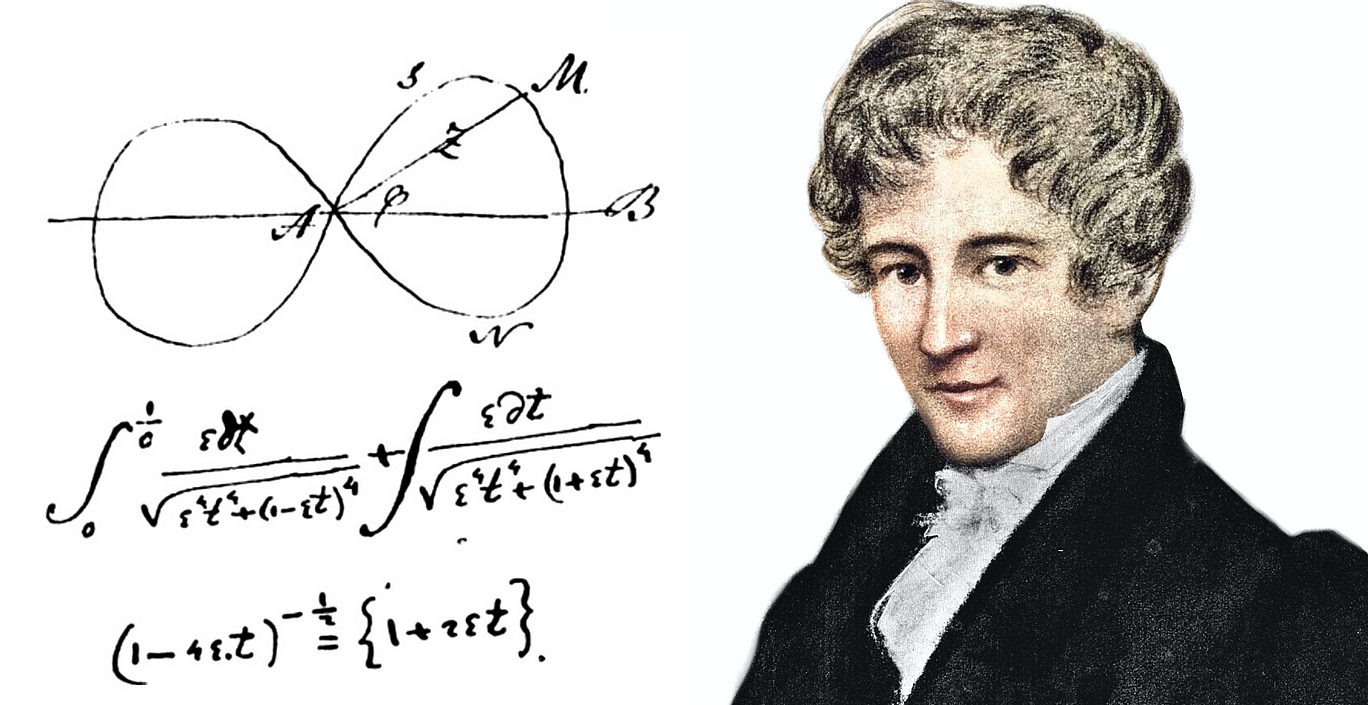
\includegraphics[scale=.14]{Pictures/nielsabel.png}}
\caption{Niels Henrik Abel. (Johan Gørbitz, 1826)}
\label{fig}
\end{figure}
\end{frame}



% YARNE THIJS :D
\section{Introducing the Research}
%\subsection{PDE's}
\begin{frame}{Partial Differential Equations (PDE's)}
    \begin{kulblock}{Definition}
        With $u:(\Omega,\mathbb{R}) \to Y:(x,t) \mapsto u(x,t), \Omega \subseteq \mathbb{R}^n$
    
        Now find $u$, that satisfied certain conditions on it's derivatives. 
    \end{kulblock}

    Example: $\begin{cases}
        \frac{\partial u}{\partial t} + a \frac{\partial u}{\partial x} = u & \text{ for } x \in \mathbb{R}, \, t > 0 \\
		u(x,0) = x_0 (x) & \text{ for } x \in \mathbb{R} \\
    \end{cases}$
    
\end{frame}
\begin{frame}{Parabolic Partial Differential Equation}
    \centering

    $$A u_{xx} + 2B u_{xy} + C u_{yy} + D u_x + E u_y + F u + G = 0$$

    Parabolic: $B^2 - AC = 0$\\

    \vspace{8mm}

    Example (Heat equation): $\frac{\partial u}{\partial t} = \alpha \frac{\partial^2 u}{\partial x^2}$

    But more with Fien in the financial application

\end{frame}
\begin{frame}{Elliptic Partial Differential Equation}
    \begin{itemize}[<+->]
        \item 2 dimensions: $\Omega \subset \mathbb{R}^2$

            $$A u_{xx} + 2B u_{xy} + C u_{yy} + D u_x + E u_y + F u + G = 0$$

            Elliptic: $B^2 - AC < 0$

            $$u_{xx} + u_{yy} + \text{lower orders} = 0$$
            
        \item $2 \leqslant n$ dimensions: $\Omega \subset \mathbb{R}^n$

            $$L u = \sum_{i=1}^n \sum_{j=1}^n a_{ij} \frac{\partial^2 u}{\partial x_i \partial x_j} + \dots = 0$$

            Elliptic: The eigenvalues are all positive or all negative
    \end{itemize}
\end{frame}


\begin{frame}{An example: Laplace' s Equation}
    $$\nabla^2 f = 0 = \Delta f$$

    2 dims, independent, rectangular: $\frac{\partial^2 u}{\partial x^2} + \frac{\partial^2 u}{\partial y^2} = 0 = u_{xx} + u_{yy}$

    \begin{itemize}
        \item Rectangular Coordinates: \hfill $\nabla^2 f = \frac{\partial^2 f}{\partial x^2} + \frac{\partial^2 f}{\partial y^2} + \frac{\partial^2 f}{\partial z^2} = 0$
        \item Cylindrical Coordinates: \hfill $\nabla^2 f = \frac{1}{r} \frac{\partial}{\partial r} \left( r \frac{\partial f}{\partial r} \right) + \frac{1}{r^2} \frac{\partial^2 f}{\partial \theta^2} + \frac{\partial^2 f}{\partial z^2} = 0$
        \item Spherical Coordinates: \hfill $\nabla^2 f = \frac{1}{r^2} \frac{\partial}{\partial r} \left( r^2 \frac{\partial f}{\partial r} \right) + \frac{1}{r^2 \sin \theta} \frac{\partial}{\partial \theta} \left(\sin \theta \frac{\partial f}{\partial \theta}\right) + \frac{1}{r^2 \sin^2 \theta}\frac{\partial^2 f}{\partial \phi^2} = 0$
    \end{itemize}
\end{frame}
% \subsection{Regularity}
\begin{frame}{What is Regularity?}
    % https://math.stackexchange.com/questions/2372091/definition-of-regularity-in-pde-theory

    \pause 
    \begin{center}
        Left as exercise to the audience! 
    \end{center}

    \pause 

    \begin{kulblock}{Wikipedia \hfill {\tiny \link{https://en.wikipedia.org/wiki/Regularity\_theory}}}
    
        Regularity is a property of elliptic partial differential equations such as Laplace's equation. Hilbert's nineteenth problem was concerned with this concept
    \end{kulblock}

    % Wat denken  jullie dat de definitie is? Nah-uh, is gewoon vaag begrepen :D
\end{frame}




\section*{\phantom{}}
% Outro And Q&A page Lol
\begin{nonumberframe}
    \titlepage
\end{nonumberframe}


\end{document}